\chapter{Datos}
\label{chapter:datos}

\section{Etapas de producción de la EFF}
\label{section:etapas_eff}

En este proyecto se utiliza información tanto de las respuestas al cuestionario de la EFF, como del paradata recopilado durante la producción de los datos. Para poder comprender mejor esos datos es importante conocer las etapas de este proceso de producción y los ficheros de datos que se generan durante cada una. En la Figura \ref{fig:eff_phases} puede observarse un resumen de este proceso. La producción de la EFF se divide en dos grandes fases: Campo y Post-Campo. Durante el Campo se contacta con los hogares, se realizan las entrevistas personales, se procesan los datos y se realiza parte de la revisión de los mismos. En el Post-Campo se termina el proceso de revisión, se evalúa el grado de no-respuesta de los datos de cada hogar para eliminar las entrevistas con poco contenido informativo, y se procede a la imputación de la no-respuesta. Tras este último proceso, se obtienen los datos finales.

\begin{figure}[ht]
	\centering
	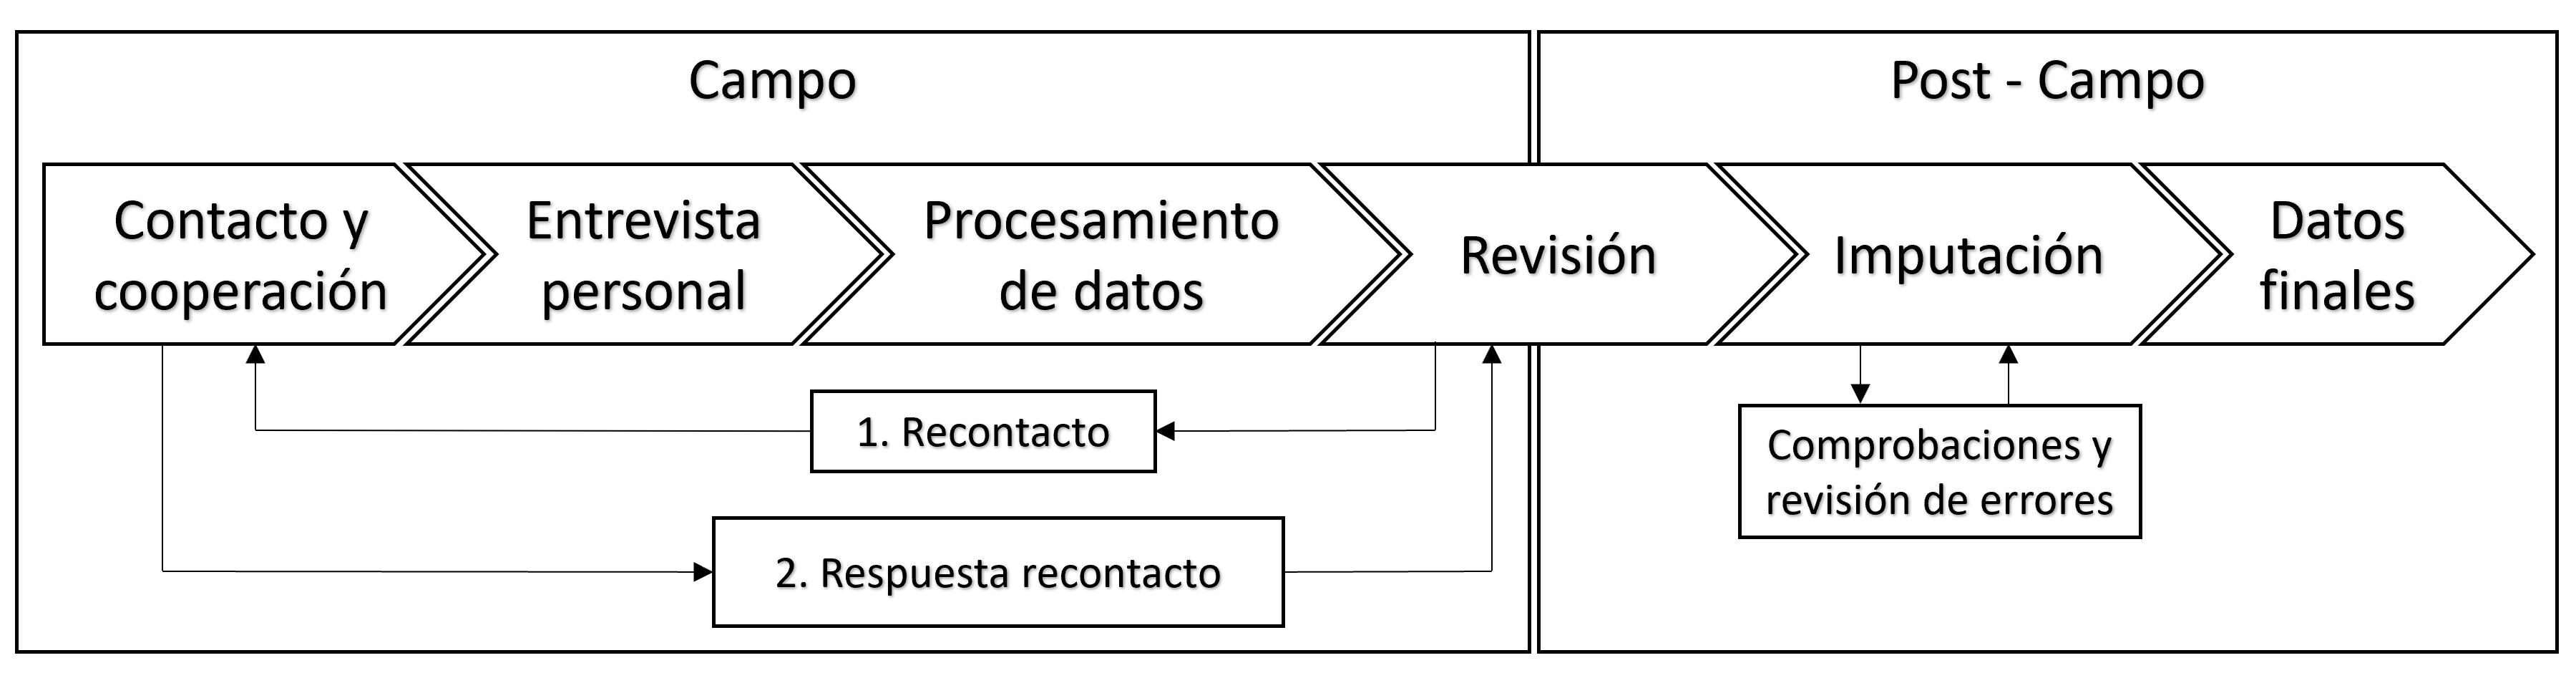
\includegraphics[width=1\textwidth]{figs/fases_creacion_datos_eff.png}
	\caption{Fases de la creación de datos de la EFF}
	\label{fig:eff_phases}
\end{figure}

A continuación se hace una breve descripción de los aspectos más relevantes de las subfases y que son importantes para la selección de variables para este estudio.

\begin{itemize}
    \item \textbf{Contacto y cooperación:} Se envía una carta a los hogares para informar sobre su selección para la encuesta y que una persona les visitará personalmente en su domicilio para hacerles una entrevista personal. El contacto puede requerir varias visitas, ya que es necesario que algún miembro del hogar esté físicamente en su hogar cuando tenga lugar la visita presencial. La información sobre cada intento (fecha y hora, resultado...) se recoge en un ordenador. Antes de establecer el contacto, los entrevistadores rellenan un cuestionario que recoge información sobre las características del barrio y del edificio en el que vive el hogar. Los entrevistadores también llevan documentación sobre la encuesta que pueden utilizar para intentar convencer al hogar, como por ejemplo un folleto con noticias de prensa en las que se ha hablado de la EFF.
    \item \textbf{Entrevista personal:} Se realiza una entrevista personal a la persona con más conocimiento de las finanzas del hogar, que se denomina Persona de Referencia o PR. La PR puede ser miembro del hogar, o un representante del mismo, demoninado proxy, siempre y cuando sea la persona con mayor conocimiento de las finanzas del hogar. También pueden participar otros miembros del hogar. Las entrevistas suelen durar entre una hora y hora y media (\cite{effmethod2017}). Antes de empezar la entrevista, se pide a la PR su consentimiento para que algunas partes de la misma puedan ser grabadas en audio por motivos de calidad de los datos. La entrevista puede realizarse aunque no haya grabación. Los entrevistadores recogen las respuestas en un ordenador o una tablet (CAPI), y también pueden anotar en comentarios de texto todos los detalles que consideren importantes para la revisión. La PR puede decidir no contestar a ciertas preguntas. Su valor se asignará como missing, y se imputará más adelante. Las cantidades monetarias pueden responderse en valor puntual, o dentro de un rango de valores. Tras la entrevista, y sin la presencia de los hogares, los entrevistadores rellenan un cuestionario con información sobre el desarrollo de la entrevista, en el que por ejemplo se recoge el nivel de comprensión de la PR a las preguntas, el nivel de interés mostrado por la PR o cuántas personas han participado en la entrevista.
    \item \textbf{Procesamiento de datos:} Los ordenadores y servidores de la empresa de campo procesan los datos recogidos durante el contacto con los hogares y durante las entrevistas. Se crean tres ficheros, uno con las respuestas al cuestionario, uno con la información de los contactos con cada hogar, y finalmente uno con la información del paradata recogido por el ordenador durante la entrevista\footnote{También se crea un fichero con los comentarios de texto recogidos por los entrevistadores durante la entrevista, pero no se ha podido incluir en este estudio por falta de tiempo.}.
    \item \textbf{Revisión:} Un equipo de personas revisa individualmente todas las entrevistas y corrige los errores que puedan detectarse. Si hay información relevante que se ha recogido erróneamente o se ha omitido, se contacta de nuevo con el hogar para corregirlo o recuperar esa información. Este recontacto se hace por teléfono. Toda la información sobre la revisión (cambios sobre variables, recontactos...) se recoge en una aplicación informática y puede ser exportada en ficheros de diversos formatos (csv, excel...).
    \item \textbf{Imputación:} Se analiza la proporción de preguntas sin responder dentro de cada entrevista (no-respuesta), y se eliminan las que no superen ciertos umbrales de calidad. Todas las variables que contienen no-respuesta se imputan mediante técnicas de imputación múltiple\footnote{Los métodos de imputación múltiple utilizados en la EFF pueden consultarse en \cite{barcelo2006imputation}.}. Se crean 5 ficheros con datos imputados.
\end{itemize}

Con respecto a los procedimientos de Contacto y Entrevista personal, es necesario mencionar que algunos elementos tuvieron que modificarse durante la EFF2020, ya que el campo tuvo lugar entre noviembre de 2020 y junio de 2021, y se vió afectado por la pandemia del Covid-19. Durante esa ola, los entrevistadores siguieron visitando personalmente a los hogares para conseguir su colaboración\footnote{Durante el principio del campo, algunos hogares panel fueron contactados sólo por teléfono, pero a las pocas semanas se decidió establecer la visita personal como el procedimiento estándar.}, pero siempre respetando las medidas de distanciamiento social. Las entrevistas se realizaron de manera telefónica asistida por una tablet (CATI). El resto de procedimientos se mantuvieron como en otras ediciones.

Para la elaboración de este proyecto se utiliza la información recopilada durante las olas de la EFF2017, EFF2020 y EFF2022 \footnote{En el momento de escribir este documento, la EFF2022 se encontraba en pleno proceso de imputación, por lo que el equipo del Banco de España ya conocía los resultados de participación de esa ola y era posible utilizarlos para este proyecto.}. Estas ediciones son las únicas que cuentan con la información más detallada de paradata y de las características de los entrevistadores. En ediciones anteriores esta información o no está disponible, o contiene errores de medida que no son fácilmente corregibles. A pesar de esto, es posible identificar en cuántas ediciones ha participado cada hogar, por lo que es posible utilizar información que se remonta hasta la edición de la EFF2011. Los ficheros de datos que se utilizan durante este proyecto son:

\begin{itemize}
    \item \textbf{Fichero de trabajo:} Registro de hogares con entrevistas válidas. Hay uno para cada edición de la encuesta. Contiene la información de las respuestas de los hogares, incluyendo las correcciones y ediciones de la revisión. Se indican los datos que deben ser imputados. También incluye variables auxiliares generadas para el proceso de imputación (características del hogar, de los miembros, del municipio...) y contadores de no respuesta de cada entrevista. Es el fichero que se utiliza para imputar. Se utilizan dos ficheros, el de la EFF2017 y el de la EFF2020.
    \item \textbf{Fichero de datos imputados:} Registro de hogares que contiene las respuestas al cuestionario después de haber imputado los datos con no-respuesta de los hogares. Hay cinco ficheros para cada edición, pero por simplicidad sólo se utiliza uno de los conjuntos de datos de la imputación multiple. Sólo contiene variables imputadas e indicadores de las características del hogar. Se utilizan dos ficheros, los de EFF2017 y EFF2020.
    \item \textbf{Fichero de contactos:} Registo de hogares contactados durante una ola de la EFF. Hay uno para cada ola de la EFF. Contiene información sobre el número de intentos de contacto con cada hogar, la fecha en que se produjo, el resultado de cada uno de ellos (aplazamientos, rechazos...) y las respuestas al cuestionario de vecindario rellenado por los entrevistadores. Se utilizan tres ficheros, los de EFF2017, EFF2020 y EFF2022.
    \item \textbf{Fichero de revisión:} Registro de incidencias durante el proceso de revisión y los recontactos. hay uno para cada edición de la EFF. Contiene información general sobre el proceso de revisión (por ejemplo, si se ha realizado un recontacto), y el resto de registros son incidencias en los datos que se detectado (por ejemplo, si se ha omitido una propiedad inmobiliaria, se abrirá un registro indicando esa incidencia y cómo se ha solucionado). Se utilizan dos ficheros, los de EFF2017 y EFF2020.
    \item \textbf{Fichero de paradata:} Registro de las pantallas visualizadas durante el uso del software CAPI durante cada entrevista. Hay uno para cada edición de la EFF. Cada registro es una pantalla visualizada durante una entrevistacada entrevista y se recoge cómo fue la interacción del entrevistador con el ordenador en esa pantalla durante la entrevista. En concreto, contiene la fecha y hora en la que se cargó la pantalla, si se pasó a la pantalla siguiente (se dió una respuesta), el tiempo que se estuvo visualizando dicha pantalla, si se volvió a la pantalla anterior o incluso si se seleccionó parar la entrevista en esa pantalla. Si en una entrevista se pasó varias veces por una pantalla, esa pantalla tendrá tantos registros como veces se cargó esa pantalla. Es posible agrupar los registros por entrevista, pregunta o sección, y ver el flujo de pantallas que se siguió durante la entrevista. Se utilizan dos ficheros, los de EFF2017 y EFF2020.
    \item \textbf{Censo de entrevistadores:} Registro de entrevistadores que contiene la información disponible sobre los entrevistadores que han participado desde la EFF2014 a la EFF2022. Sólo hay un fichero.
\end{itemize}

\section{Análisis Exploratorio de los Datos}
\label{section:exploring}

El objetivo del análisis exploratorio de datos es investigar las características de los datos que se van a utilizar. Por un lado, se observan las características particulares de cada variable, y por otro las relaciones que existan entre ellas, y de manera especial la que tienen con la variable Attrition. Esta información es importante porque ayuda a identificar y tratar rasgos de las variables que pueden afectar a los modelos de machine learning que se quieren entrenar.

Como veremos a continuación, en este proyecto se ha manejado una gran cantidad de datos de gran diversidad de origen y formato. El análisis exploratorio de toda esa información es muy amplio y no es posible incluir todo el trabajo en esta sección. Por esa razón, sólo se muestran resultados que son de interés para el análisis del panel attrition, o resultados que han ayudado a la toma de decisiones para la selección o transformación de variables para los modelos de predicción. 

Este análisis se separa en cinco bloques. El primero describe la gran cantidad de datos que se generan en la EFF y el proceso de filtrado que se ha realizado para este proyecto. Los tres boques siguientes abordan tres temas que preocupan a los productores de encuestas porque suelen afectar a la participación de los panelistas: la experiencia en la encuesta y las entrevistas, la persona que responde a la encuesta, y las características de los hogares. Finalmente, se aborda el problema de valores atípicos detectados en las duraciones de las entrevistas.

\subsection*{Número de registros y variables}
\label{section:registers_variables}

Una sola edición de la EFF produce una gran cantidad de datos. El Cuadro \ref{table:registers} muestra el número de registros y variables disponibles en cada uno de los ficheros utilizados en este proyecto. Estos números incluyen a todos hogares contactados y a todas variables generadas durante la producción de datos de la EFF en sus ediciones de 2017, 2020 y 2022\footnote{De la EFF2022 sólo se utiliza el fichero de contactos ya que sólo se necesita la información sobre la participación de los hogares panel en dicha edición.}. Tras realizar el filtrado de hogares elegibles para el estudio, se obtiene que los hogares de la EFF2017 elegibles para la EFF2020 son 5,937\footnote{Originalmente se identificaron 5938 hogares de la EFF2017 elegibles para la EFF2020. Pero uno de esos hogares no tenía registros en el fichero de paradata, y se eliminó del conjunto de datos final.} y los hogares elegibles de la EFF2020 para la EFF2022 son 5,505. Con respecto al censo de entrevistadores, sus números incluyen a los 260 entrevistadores que han participado en las ediciones de 2014, 2017, 2020 y 2022. Tras filtrar por las ediciones de 2017 y 2020, se obtiene que en la EFF2017 participaron 69 entrevistadores, mientras que en la EFF2020 participaron 65 entrevistadores, de los cuales 25 personas también participaron en la EFF2017.

\begin{table}[ht]
\centering{}
\begin{tabular}{lcccc}
\cline{2-5}
                            & \multicolumn{2}{c}{\textbf{EFF2017}}        & \multicolumn{2}{c}{\textbf{EFF2020}}        \\ \cline{2-5} 
\textbf{Nombre del fichero} & \textbf{Registros}   & \textbf{Variables}   & \textbf{Registros}   & \textbf{Variables}   \\ \hline
Fichero de trabajo          & 6,413                & 6,103                & 6,313                & 6,497                \\
Fichero de datos imputados  & 6,413                & 659                  & 6,313                & 787                  \\
Fichero de contactos        & 14,456               & 640                  & 15,457               & 636                  \\
Fichero de revisión      & 44,760               & 22                   & 35,217               & 51                   \\
Fichero paradata            & 2,807,091            & 13                   & 3,121,437            & 12                   \\ \hline
                            & \multicolumn{1}{l}{} & \multicolumn{1}{l}{} & \multicolumn{1}{l}{} & \multicolumn{1}{l}{} \\
                            & \multicolumn{4}{c}{\textbf{EFF2022}}                                                      \\ \cline{2-5} 
\textbf{}                   & \multicolumn{2}{c}{\textbf{Registros}}      & \multicolumn{2}{c}{\textbf{Variables}}      \\ \cline{2-5} 
Fichero de contactos        & \multicolumn{2}{c}{15,182}                  & \multicolumn{2}{c}{636}                     \\ \hline
                            & \multicolumn{1}{l}{} & \multicolumn{1}{l}{} & \multicolumn{1}{l}{} & \multicolumn{1}{l}{} \\
\multicolumn{5}{c}{\textbf{Censo de entrevistadores}}                                                                   \\ \hline
\multicolumn{2}{c}{\textbf{Registros}}             & \multicolumn{3}{c}{\textbf{Variables}}                             \\ \hline
\multicolumn{2}{c}{260}                            & \multicolumn{3}{c}{56}                                             \\ \hline
\end{tabular}
\caption{\textit{Número de registros y variables de los ficheros de datos}}
\label{table:registers}
\end{table}

En el cuadro \ref{table:registers} también puede observarse que hay ficheros que almacenan más de 6,000 variables. Esto supone un problema de dimensionalidad ya que hay más variables que registros en los datos. Sin embargo, hay cuatro maneras para reducir drásticamente el número de variables a manejar sin perder información relevante, y obtener las variables mencionadas en el cuadro \ref{table:vars}. La primera es que la inmensa mayoría de variables almacenan las respuestas al cuestionario principal de la EFF. En el capítulo \ref{chapter:datos} se comenta que el número de preguntas que se formulan depende del número de miembros del hogar, sus edades, y los activos y deudas que posea el hogar, y que en la EFF2017 se plantearon entre 137 y 594 preguntas a cada hogar. Como los modelos de predicción requieren de variables que contengan datos para todos los registros, es posible descartar muchas variables por no tener valores para todos los hogares.

La segunda razón para descartar variables es que muchas no son informativas en su estado original y necesitan ser combinadas con otras para poder obtener información interpretable, o se utilizan como apoyo para la imputación. Por ejemplo, la información sobre cantidades monetarias se recoge en cuatro variables que permiten declarar valores en intervalos a los hogares que no quieran o no puedan dar un valor puntual (\cite{effmethod2017}). Esto se utiliza en la imputación para estimar valores puntuales dentro del rango declarado por el hogar. Al usar el fichero de datos imputados para entrenar los modelos, todas esas variables auxiliares se descartan.

En tercer lugar, hay variables duplicadas porque están almacenadas en varios ficheros de datos, por lo que sólo es necesario extraerlas de uno de esos ficheros. Por ejemplo, todas las variables que aparecen en el fichero de datos imputados también aparecen en el fichero de trabajo. Del fichero de trabajo se extraen indicadores de no-respuesta y otras variables de interés que no aparecen en el fichero de datos imputados, y de éste último se extraen las variables con los valores missing imputados.

Finalmente, para que los modelos de predicción puedan aplicarse tanto para datos de la EFF2017 como para la EFF2020, sólo se seleccionan las variables que estaban disponibles en ambas olas. Esta tarea ha requerido una gran dedicación de esfuerzo y tiempo, ya que en algunos ficheros se detectaron variables que no mantuvieron su nomeclatura, el tipo de dato almacenado o la codificación de los datos entre diferentes olas. Para asegurar la homogeneidad, se ha revisado de manera individualizada la nomenclatura y la codificación de cada variable para ambas ediciones de la EFF.

\subsection*{La experiencia en la encuesta y las entrevistas}

En la sección \ref{section:causes_attrition} se comentó que los hogares panel poseen experiencia previa sobre la encuesta que puede afectar a su participación en olas posteriores. Esta experiencia puede abarcar varias ediciones, pero también puede ser informativo observar datos sobre la ola más reciente.

En la figura \ref{fig:fig1} hay cuatro gráficos de mekko que muestran cómo fue la participación en la EFF2020 de hogares elegibles de la EFF2017 según su ola de entrada en la EFF, si consintieron grabar la entrevista de la EFF2017, si dicha entrevista se realizó con un proxy, y el nivel de recelo que mostraron después de realizarla. Los gráficos de mekko son gráficos de columnas apiladas 100\% en los que la anchura de cada columna muestra la proporción de hogares que hay de una categoría dentro de la muestra. Las regiones superiores o rojas de cada columna muestran la proporción de hogares que no participaron en la EFF2020, mientras que las regiones inferiores o azules muestran la proporción de hogares que sí participaron.

\begin{figure}[ht]
	\centering
	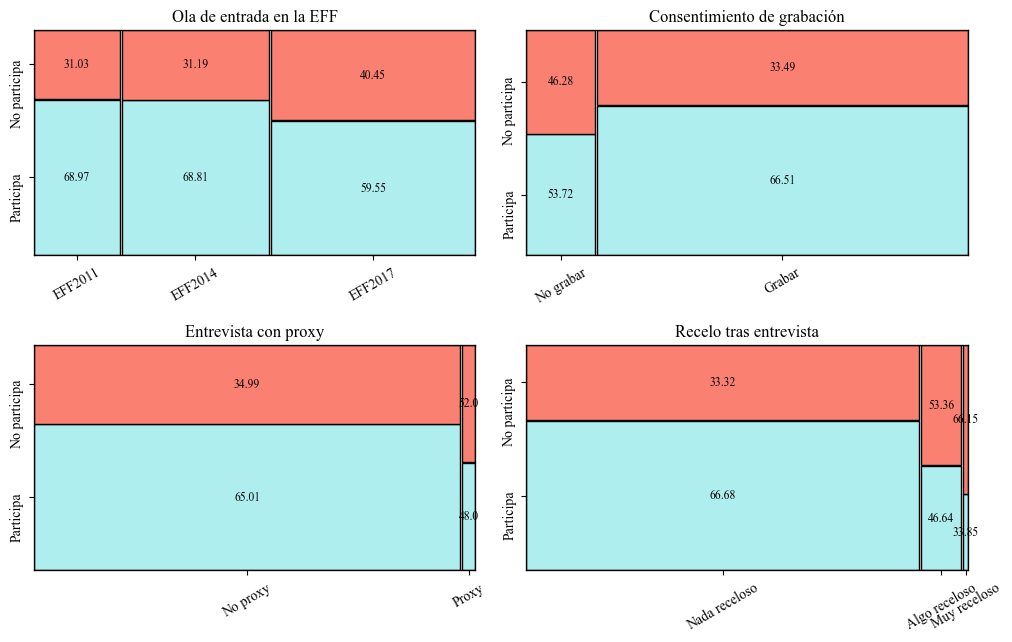
\includegraphics[width=1\textwidth]{figs/figure1.png}
	\caption{Participación en EFF2020 por experiencia en la EFF y en la entrevista de EFF2017}
	\label{fig:fig1}
\end{figure}

En la figura superior izquierda de la figura \ref{fig:fig1} se observa que la proporción de abandono de hogares que participaron por primera vez en 2017 es mayor que la de los que lo hicieron por primera vez en 2014 o en 2011, y entre estas dos últimas la proporción es similar. Esto sugiere que los hogares que van a participar en su segunda ola podrían ser más complicados de retener que los que llevan más tiempo. 

La figura superior derecha muestra que la proporción de no participación es mayor entre los hogares que no consintieron grabar la entrevista en 2017. Esto puede ser una señal de recelo hacia la encuesta, lo que puede dificultar la participación en las siguientes ediciones. En ese sentido también es interesante ver si los hogares se mostraban recelosos tras la entrevista, que es lo que se observa en la figura inferior derecha. La gran mayoría de hogares no se mostraron recelosos tras la entrevista, pero se observa que la proporción de hogares que no participaron en la EFF2020 es mayor a medida que aumenta el nivel de recelo.

Finalmente, en la figura inferior izquierda, se ve que la proporción de abandonos en 2020 fue mayor entre los hogares que hicieron la entrevista con proxy en 2017. Una situación que ha ocurrido bastantes veces en la EFF y que puede encajar con un abandono es el de un hogar formado por personas muy mayores en el que quien lleva las finanzas y termina respondiendo a la entrevista es un hijo o un familiar. Muchos de estos familiares se muestran muy recelosos y, comprensiblemente, quieren que no se moleste a sus familiares. En este tipo de situaciones puede ser más importante volver a convencer a estos familiares que a los propios miembros del hogar, ya que al final son ellos quienes conocen la información del hogar.

Algunos de estos resultados pueden parecer poco útiles porque es razonable pensar que un hogar que se mostró receloso durante la entrevista seguramente será más complicado de convencer para volver a participar en la siguiente edición. Sin embargo, para un entrevistador que está a punto de entrevistar a un hogar, puede ser muy útil saber si ese hogar se mostró receloso tras la anterior entrevista. A la hora convercer al hogar puede centrarse más en utilizar argumentos relacionados con la confidencialidad y la seguridad de los datos y no tanto en hablar de la relevancia de la encuesta o del eco que ha tenido en los medios de comunicación. Estos resultados pueden servir para justificar este tipo de análisis y encontrar qué información puede ayudar al trabajo de los entrevistadores.

\subsection*{Características y comportamiento de la PR}

En la sección \ref{section:causes_attrition} se vió que las características de la persona que responde a una encuesta puede ser relevante para el panel attrition. Es este apartado vamos a ver cómo se relacionan algunas características de la PR en 2017 con la participación del hogar en la EFF2020.

\begin{figure}[ht]
	\centering
	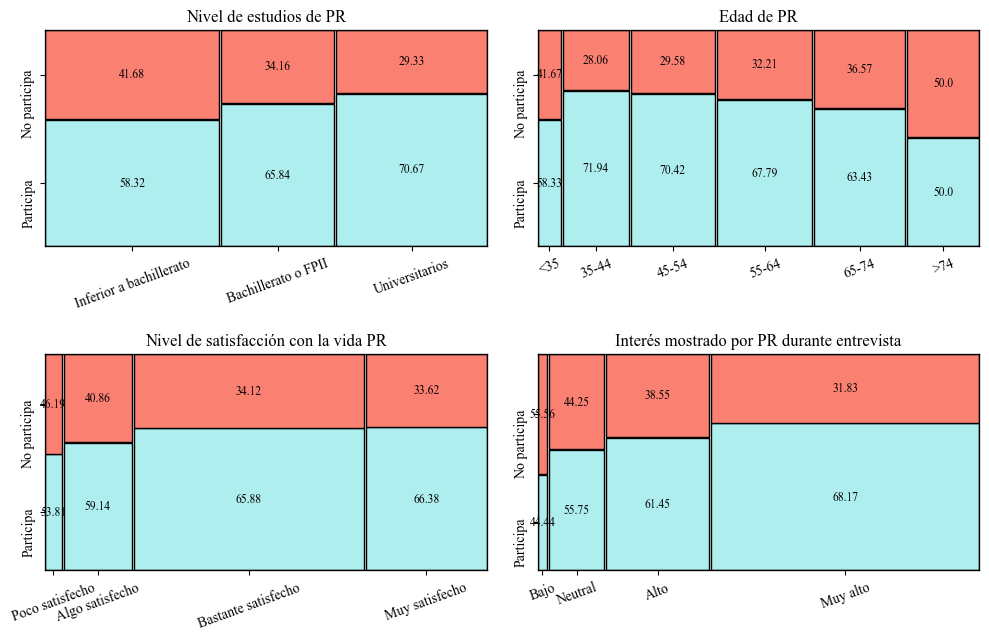
\includegraphics[width=1\textwidth]{figs/figure2.png}
	\caption{Participación en EFF2020 por características y actitudes de PR en EFF2017}
	\label{fig:fig2}
\end{figure}

La figura \ref{fig:fig2} contiene los gráficos de mekko de la participación en la EFF2020 según el nivel máximo de estudios alcanzados de la PR, su edad y su satisfacción con la vida en 2017 y el interés que mostró durante la entrevista de la EFF2017. El gráfico superior izquierdo muestra que la proporción de hogares que no participó en la EFF2020 es mayor cuanto menor era el nivel de estudios de la PR en 2017. Una posible explicación de este resultado podría deberse a la menor tenencia de productos financieros por parte de hogares de menor nivel educativo (\cite{hospido2023encuesta}). El cuestionario de la EFF contiene muchas preguntas sobre muchos productos financieros diferentes, y es razonable pensar que alguien que no posee este tipo de activos piense que no tiene sentido participar en esta encuesta. Un entrevistador con este conocimiento podría preparar un argumentario orientado a destacar que sin su participación no se podría identificar a hogares con sus características y así para poder diseñar políticas económicas específicas para esos hogares.

En el gráfico superior derecho se ve que la proporción de hogares que participó en 2020 aumenta a medida que aumenta la edad de la PR en 2017, excepto cuando ésta tenía menos de 35 años, que presenta la segunda proporción más alta de los grupos de edad. El resultado para los hogares más jóvenes podría explicarse por el hecho de que cada vez menos de estos hogares son propietarios de su vivienda principal (\cite{eff2014results}, \cite{eff2017results}, \cite{eff2020results}) y esto puede hacer que sean más propensos a mudarse, y por tanto ser más difíciles de localizar. El caso de las PR de mayor edad podría explicarse por motivos de fallecimiento.

Finalmente, en los gráficos de la parte inferior de la figura \ref{fig:fig2} vemos, por un lado, que la proporción de hogar que dejan de participar en 2020 se reduce a medida aumenta el nivel de satisfacción con la vida de la PR en 2017, y por otro, que la proporción de hogares que participaron en 2020 aumenta a medida que aumenta el interés por la encuesta. Este último resultado es razonable y útil de saber para el entrevistador porque puede basar su argumentario para convencer al hogar en ese interés.

\subsection*{Características hogar}

En este apartado se analiza a nivel exploratorio la posible relación que puedan tener las características del hogar con el panel attrition. En concreto, se analizan las variables de renta, riqueza y tenencia de deudas. La renta y la riqueza son el eje central de la EFF y es habitual incluirlas de alguna manera en cualquier análisis que se haga con los datos de la encuesta.

En la figura \ref{fig:fig3} hay tres gráficos de mekko en el que se observa la proporción de hogares que participaron en la EFF2020 según la posición relativa de cada hogar en las distribuciones de renta anual y riqueza bruta\footnote{La riqueza bruta se define como la suma del valor de todos los activos que posee el hogar (activos reales + activos financieros = riqueza bruta).} de los hogares españoles en 2017, y también si el hogar tenía deudas pendientes en 2017. La posición relativa de cada hogar dentro de la distribución de renta se muestra indicando los percentiles de la distribución total entre los que se sitúa cada hogar. Si el nivel de renta de un hogar lo sitúa entre los percentiles 60 y 80 del total de la renta de hogares en España, entonces ese hogar está en la categoría "P60-P80" de la distribución de renta, y si se sitúa por encima del percentil 90, la categoría es "\verb|>|P90".

\begin{figure}[ht]
	\centering
	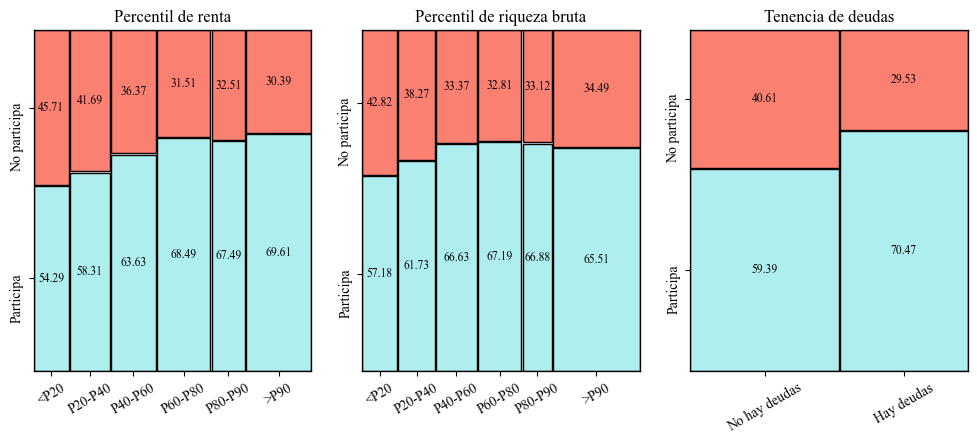
\includegraphics[width=1\textwidth]{figs/figure3.png}
	\caption{Participación en EFF2020 por renta, riqueza y tenencia de deudas en EFF2017}
	\label{fig:fig3}
\end{figure}

En el gráfico de la izquierda de la figura \ref{fig:fig3} se observan dos tendencias diferentes dependiendo del nivel de renta anual de 2017. Por encima del percentil 60 no se aprecian grandes diferencias en la proporción de panelistas que no participaron en 2020, pero por debajo de ese percentil se ve que la proporción de hogares que no participaron es mayor cuanto menor es el nivel de renta. Una posible explicación puede venir de que los niveles de tenencia de activos son menores cuanto menor es el nivel de renta de los hogares (\cite{eff2017results}) y, como se ha comentado para el nivel educativo, es razonable pensar que un hogar que tiene pocos activos considere que no tiene sentido participar en una encuesta como la EFF. Estas dos tendencias también se observan para la distribución de riqueza bruta, pero en este caso la tendencia se observa por debajo del percentil 40 de riqueza bruta. La explicación de por qué la proporción de abandonos es mayor sería similar a la de renta. Si no se tienen activos, se puede pensar que no tiene sentido participar en la EFF.

Finalmente, el gráfico de la derecha muestra la proporción de hogares que participaron en la EFF2020 según si tenían deudas pendientes en 2017. Se observa que la proporción de hogares que no participan en 2020 es mayor entre los hogares que no tenían  deudas en 2017.

\subsection*{Duración de las entrevistas}
\label{subsection:duration}

En esta última pieza de análisis exploratorio se comenta el tratamiento de valores atípicos detectados en la duración de las entrevistas. En el entrenamiento de los modelos de la sección \ref{section:evaluation_models} se ha utilizado la duración total de la entrevista en segundos. Este valor se obtiene del fichero paradata calculando, para cada hogar, la suma de los segundos que pasaron en cada pantalla del CAPI durante la entrevista. Al analizar la distribución de las duraciones se encontraron valores atípicos que indicaban que hubo entrevistas que duraron más de 20 horas, cuando las entrevistas suelen durar entre una hora y hora y media (\cite{effmethod2017}).

\begin{figure}[ht]
	\centering
	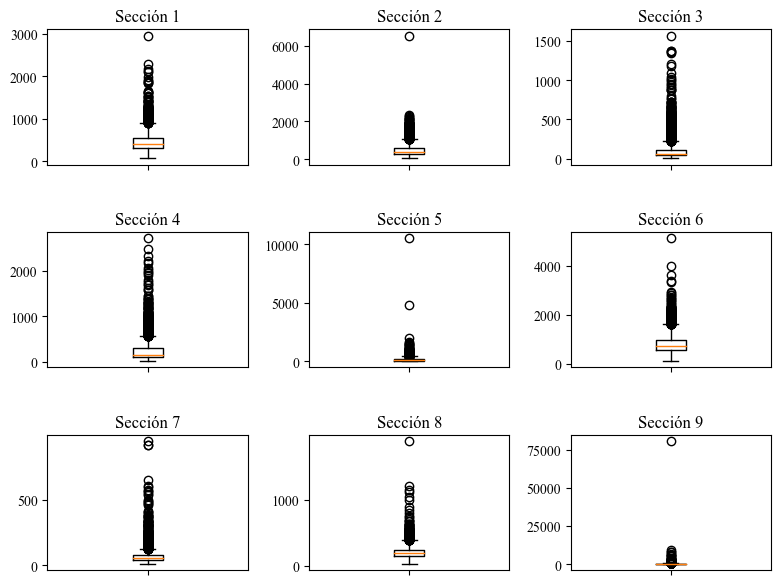
\includegraphics[width=1\textwidth]{figs/figure4.png}
	\caption{Duración por sección del cuestionario en la EFF2017}
	\label{fig:fig4}
\end{figure}

A partir de la información en el fichero paradata se calcularon las duraciones de cada una de las nueve secciones de la EFF. La figura \ref{fig:fig4} contiene los gráficos box-plot de las duraciones de las 9 secciones del cuestionario de la EFF2017. En estos gráficos se ve que hay valores atípicos en todas las secciones, y que algunos son particularmente altos, especialmente en la sección 9. Se sospecha que los entrevistadores no cerraron bien la aplicación del ordenador o la tablet al tomar un descanso, o al interrumpir una entrevista, o al terminarla.

Estos valores tan altos representan un error de medición importante que puede afectar a los modelos de predicción, por lo que es necesario tratarlos. Como hay secciones que contienen más preguntas que otras, la duración en cada sección dependerá de cuántas preguntas se formulen en cada sección. Como el fichero paradata contiene esa información, se decide imputar la duración a nivel de sección, y en concreto se imputan los valores que estén por encima del percentil 99.9 de la duración de dicha sección. Se utiliza el algoritmo kNN (\textit{k-nearest neighbors}) con k=5 y distancia euclídea. Como rasgos de cada sección se calculan el número de preguntas que se formulan una sola vez, el número total de preguntas formuladas, el número de veces que se vuelve a una pantalla anterior, el número de paradas, el número de preguntas categóricas con 1-4 opciones de respuesta, 5-9 opciones de respuesta o más de diez opciones de respuesta, y el tiempo pasado en preguntas monetarias. Tras la imputación, se calcula la duración total de la entrevista como la suma de las duraciones de todas las secciones. Este procedimiento se implementa por separado para las duraciones de cada ola.